\documentclass[main]{subfiles} 

\begin{document}

\chapter{REVIEW OF RELATED LITERATURES}

\section{Basic OOP Concepts}
\subsection{Introduction}
C++, as we all know is an extension to C language and was developed by Bjarne Stroustrup at Bell Labs. C++ is an intermediate level language, as it comprises a confirmation of both high level and low level language features. C++ is a statically typed, free form, multiparadigm, compiled general-purpose language.

It is an Object Oriented Programming language but is not purely Object Oriented. Its features like \texttt{friend} and \texttt{virtual} violate some of the very important OOP concepts such as data hiding, rendering this language unworthy of being called completely Object Oriented.


\subsection{Structure of Code}
A C++ program is structured in a specific and particular manner. In C++, a program is divided into the following three sections:
\begin{itemize}
    \item\textbf{Standard Libraries Section}
    \item\textbf{Class Definition Section}
    \item\textbf{Functions Definition Section}
    \item\textbf{Main Function Section}
\end{itemize}

For example, let us look at the implementation of the Hello World program:
\begin{minted}[bgcolor=lightgray, breaklines]{cpp}
#include <iostream>
#include <string>

//using namespace std;
class PrintText{
 public:
    PrintText(std::string);
}

PrintText::PrintText(std::string txt){
    std::cout << txt << std::endl;
}

int main() {
  PrintText text("Hello World!");
  return 0;
}
\end{minted}

\textbf{Standard Libraries Section}
\begin{minted}[bgcolor=lightgray, breaklines]{cpp}
#include <iostream>
#include <string>
//using namespace std;
\end{minted}
\begin{itemize}
    \item\texttt{\#include} is a specific preprocessor command that effectively copies and pastes the entire text of the file, specified between the angle brackets, into the source code. This file is also called header file.
    
    \item The file \texttt{<iostream>} is merely for input-output streams. This header file contains code for console input and output operations. This file is a part of \texttt{std} namespace.
    
    \item The other header file \texttt{<string>} is used for string related functions and is also a part of \texttt{std} namespace.
    
    \item \texttt{namespace} is a prefix that is applied to all the names in a certain set. For example, \texttt{iostream} file is defined in a set what we call \texttt{std}
    and it defines two names used in this program - \texttt{cout} and \texttt{endl}.
    
    \item If \texttt{using namespace std;} is used, the compiler understands that the names like \texttt{cout} and \texttt{endl} of the \texttt{std} namespace are being used.
    
\end{itemize}

\textbf{Class Definition Section}
\begin{minted}[bgcolor=lightgray, breaklines]{cpp}
class PrintText{
 public:
    PrintText(string);
}
\end{minted}
The classes are used to map real world entities into programming. The classes are key building blocks of any C++ program. A C++ program may include several class definitions. This is the section where we define all of our classes.

In above program \texttt{PrintText} is the class and \texttt{text} is its object.

\textbf{User-defined Function Definition Section}
\begin{minted}[bgcolor=lightgray,breaklines]{cpp}
PrintText::PrintText(std::string txt){
    std::cout << txt << std::endl;
}
\end{minted}

C++ allows the programmer to define their own function. A user-defined function groups code to perform a specific task and that group of code is given a name (identifier). When the function is invoked from any part of the program, it executes the codes defined in the body of the function.

In this program the function \texttt{PrintText} is a special member function called \textit{constructor} of the class \texttt{PrintText}.

\textbf{Main Function Section}
\begin{minted}[bgcolor=lightgray, breaklines]{cpp}
    int main() {
        PrintText text("Hello World!");
        return 0;
    }
\end{minted}

\texttt{main()} function is the function called when any C++ program is run. The execution of all C++ programs begins with the \texttt{main()} function and also ends with it, regardless of where the function is actually located within the code.


\subsection{Features Of OOP}
C++ is a \textbf{general-purpose} programming language that was developed as an enhancement of the C language to include object-oriented paradigm \cite{geeksforgeeks_2020_features}. It is an imperative and a compiled language. Some of its main features are:

\begin{itemize}
    \item\textbf{Namespace:} A namespace is a declarative region that provides a scope to the identifiers (the names of types, functions, variables, etc) inside it. Namespaces are used to organize code into logical groups and to prevent name collisions that can occur especially when the code base includes multiple libraries.
    
    The following example shows a namespace declaration and method to access the member of the namespace from outside it.

    \begin{minted}[bgcolor=lightgray, breaklines]{cpp}
    namespace ContosoData{
    class ObjectManager{
    public:
        void DoSomething() {}
    };
    }
    \end{minted}

    The most convenient method to access its member is:
    \begin{minted}[bgcolor=lightgray, breaklines]{cpp}
    ContosoData::Objectmanager mgr;
    mgr.DoSomething();
    \end{minted}
     
    \item\textbf{Inheritance:} Inheritance is a process in which one object acquires some (or all) of the properties and behaviors of its parent object automatically. In such way, one can reuse, extend or modify the attributes and behaviors which are defined in other classes, from existing classes.
    
    The class which inherits the members of another class is called derived class and the class whose members are inherited is called base class. The derived class is the specialized class for the base class.
    The syntax for derived class is:
    \begin{minted}[bgcolor=lightgray, breaklines]{cpp}
    class derived_class :: visibility-mode base_class  
    {  
    // body of the derived class.  
    }  
    \end{minted}
    
    There are three visibility modes in which a derived class inherits from its base class. They are private, public and protected. Following table clarifies the concept:
    \begin{center}
    \begin{table}[H]
        \begin{tabular}{|c|c|c|c|}
            \hline
            \textbf{Base member Access Specifier} & \multicolumn{3}{|c|}{\textbf{Visibility Mode}}  \\
             & \textbf{private} & \textbf{public} & \textbf{protected} \\
             \hline
             \textbf{private} & Not Accessible & Not Accessible & Not Accessible \\
             \hline
             \textbf{public} & private & public & protected \\
             \hline
             \textbf{protected} & private & protected & protected \\
             \hline
            
        \end{tabular}
        \caption{Visibility modes}
        \label{tab:Visibility modes}
    \end{table}
    \end{center}
    
    \item\textbf{Polymorphism:}The word polymorphism means having many forms. In simple words, we can define polymorphism as the ability of a message to be displayed in more than one form. Polymorphism is considered as one of the important features of Object Oriented Programming.
    
    In C++ polymorphism is mainly divided into two types:
    \begin{itemize}
        \item Compile time Polymorphism
        \item Runtime Polymorphism
    \end{itemize}
    
    \begin{figure}[H]
        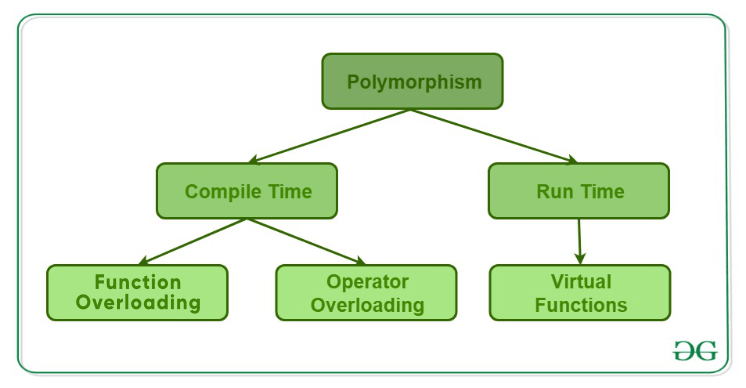
\includegraphics[width=\textwidth]{graphics/Polymorphism-in-CPP.png}
        \caption{Types of Polymorphism}
        \label{fig:Polymorphism}
        \caption*{Source: \href{https://www.geeksforgeeks.org/}{GeeksForGeeks}}
    \end{figure}
    
    
    \begin{enumerate}
        \item \textbf{Compile time Polymorphism:} This type of polymorphism is achieved by function overloading or operator overloading.
        \begin{itemize}
            \item\textbf{Function Overloading:} When there are multiple functions with same name but different parameters then these functions are said to be overloaded. Functions can be overloaded by change in number of arguments or/and change in type of arguments.
            \begin{minted}[bgcolor=lightgray, breaklines]{cpp}
#include <iostream> 
class FunOver { 
    public: 
    // function with 1 int parameter 
    void func(int x) { 
        std::cout << "value of x is " << x << endl; 
    } 
      
    // function with same name but 1 double parameter 
    void func(double x) { 
        std::cout << "value of x is " << x << endl; 
    } 
      
    // function with same name and 2 int parameters 
    void func(int x, int y) { 
        std::cout << "value of x and y is " << x << ", " << y << endl; 
    } 
}; 
  
int main() { 
    FunOver obj1; 
    // Which function is called will depend on the
    //parameters passed 
    obj1.func(7); // The first 'func' is called
    obj1.func(9.132); // The second 'func' is called 
    obj1.func(85,64); // The third 'func' is called 
    return 0; 
}  
Output:
            \end{minted}
            In the above example, a single function named func acts differently in three different situations which is the property of polymorphism.
            \item\textbf{Operator Overloading:} C++ also provide option to overload operators. For example, we can make the operator (‘+’) for string class to concatenate two strings. We know that this is the addition operator whose task is to add two operands. So a single operator ‘+’ when placed between integer operands , adds them and when placed between string operands, concatenates them.
            \begin{minted}[bgcolor=lightgray, breaklines]{cpp}
#include<iostream> 
class Complex { 
private: 
    int real, imag; 
public: 
    Complex(int r = 0, int i =0)  {
        real = r;   imag = i;
    }  // This is automatically called when '+' is used between two Complex objects 
    
    Complex operator + (Complex const &obj) { 
         Complex res; 
         res.real = real + obj.real; 
         res.imag = imag + obj.imag; 
         return res; 
    } 
    void print() { 
        std::cout << real << " + i" << imag << endl; 
    } 
}; 
   
int main() 
{ 
    Complex c1(10, 5), c2(2, 4); 
    Complex c3 = c1 + c2; // An example call to 
                          //"operator+" 
    c3.print(); 
    return 0;
}
            \end{minted}
            In the above example the operator ‘+’ is overloaded. The operator ‘+’ is an addition operator and can add two numbers(integers or floating point) but here the operator is made to perform addition of two imaginary or complex numbers.
        \end{itemize}
        \item\textbf{Runtime Overload:} This type of polymorphism is achieved by Function Overriding.
        \begin{itemize}
            \item \textbf{Function Overriding} on the other hand occurs when a derived class has a definition for one of the member functions of the base class. That base function is said to be overridden.
            \begin{minted}[bgcolor=lightgray, breaklines]{cpp}
#include <iostream> 
class base { 
public: 
    virtual void print () { 
        std::cout << "print base class" << std::endl; } 
    void show () {
        std::cout << "show base class" << std::endl; } 
}; 
   
class derived:public base { 
public: 
    void print () //print () is already virtual function in derived class, we could also declared as virtual void print () explicitly 
    { std::cout << "print derived class" << std::endl; } 
   
    void show () 
    { std::cout << "show derived class" << std::endl; } 
}; 
  
//main function 
int main()  
{ 
    base *bptr; 
    derived d; 
    bptr = &d; 
       
    //virtual function, binded at runtime (Runtime polymorphism) 
    bptr->print();  
       
    // Non-virtual function, binded at compile time 
    bptr->show();  
  
    return 0; 
} 
            \end{minted}
            Runtime polymorphism is achieved only through a pointer (or reference) of base class type. Also, a base class pointer can point to the objects of base class as well as to the objects of derived class. In above code, base class pointer ‘bptr’ contains the address of object ‘d’ of derived class.
            
            Late binding(Runtime) is done in accordance with the content of pointer (i.e. location pointed to by pointer) and Early binding(Compile time) is done according to the type of pointer, since print() function is declared with virtual keyword so it will be bound at run-time (output is print derived class as pointer is pointing to object of derived class ) and show() is non-virtual so it will be bound during compile time(output is show base class as pointer is of base type ).
        \end{itemize}
    \end{enumerate}
    \item\textbf{Templates:} A template is a simple and yet very powerful tool in C++. The simple idea is to pass data type as a parameter so that we don’t need to write the same code for different data types. For example, a software company may need sort() for different data types. Rather than writing and maintaining the multiple codes, we can write one sort() and pass data type as a parameter.
        
    C++ adds two new keywords to support templates: ‘template’ and ‘typename’. The second keyword can always be replaced by keyword ‘class’.
        
\end{itemize}


\section{Smart Pointer}
\subsection{Introduction}
Smart pointers are used to make sure that an object is deleted if it is no longer used (referenced). They are the classes wrapped around a normal pointer where the normal pointer operators like * and -> are overloaded. Using smart pointers we can make pointers work in a way that we do not need to explicitly call delete. It is a feature in C++ which is influenced by Simula's approach of memory management\cite{smart_pointers_cppref}. There are different types of smart pointers that are used for different purposes. Following are the different types of smart pointers used in this project:
\begin{itemize}
    \item Unique Pointer (\texttt{unique\_ptr})
    \item Shared Pointer (\texttt{shared\_ptr})
\end{itemize}

\subsection{Types}
\subsubsection{Unique Pointer (\texttt{unique\_ptr})}
Unique pointer is a smart pointer that was introduced in C++11 and is defined in the header \texttt{<memory>}. Unique pointer makes sure that only one copy of the pointer is possible at a given state. Unique pointer makes sure that only one pointer can point to the object at a time. It prevents the copy of the contained pointer as copy constructor and assignment operators are explicitly removed\cite{smart_pointers_wikipedia}. But \texttt{std::move} can be used to transfer the ownership from one pointer to another. After the moving of the pointer is done, the previous pointer cannot make reference to the object. The following program is an example of the use of \texttt{unique\_ptr}\cite{smart_pointers_geeksforgeeks}:

\begin{minted}[bgcolor=lightgray, breaklines]{cpp}
std::unique_ptr<int> p1(new int(5));

std::unique_ptr<int> p2 = p1;  // Compile error.

std::unique_ptr<int> p3 = std::move(p1);  
// Transfers ownership. p3 now owns the memory and p1 is set to nullptr.

p3.reset();  // Deletes the memory.
p1.reset();  // Does nothing.
\end{minted}

\subsubsection{Shared Pointer (\texttt{shared\_ptr})}
Shared pointer is also a smart pointer that was introduced in C++11 and is defined in the header \texttt{<memory>}. The shared pointer is a reference counting smart pointer that can be used to store and pass a reference beyond the scope of a function. This is particularly useful in the context of OOP, to store a pointer as a member variable and return it to access the referenced value outside the scope of the class. While \texttt{shared\_ptr} is used, it also maintains a reference counter to count the number of pointers that refers to the same object. C++11 also introduces \texttt{std::make\_shared( )} method to safely conduct the dynamic allocation the memory to the shared pointer. The following program is an example of the use of \texttt{shared\_ptr}\cite{smart_pointers_geeksforgeeks}:

\begin{minted}[bgcolor=lightgray, breaklines]{cpp}
std::shared_ptr<int> p0 = std::make_shared<int> (5);
// Valid, allocates 1 integer and initialize it with value 5.

std::shared_ptr<int[]> p1(new int[5]);
// Valid, allocates 5 integers.

std::shared_ptr<int[]> p2 = p1;  // Both now own the memory.

p1.reset();  // Memory still exists, due to p2.
p2.reset();  // Frees the memory, since no one else owns the memory
\end{minted}

\section{SFML}
\subsection{Introduction}
SFML stands for Simple and Fast Multimedia Library. This is a framework written in C++ and is based on OpenGL for its graphical rendering part. 
SFML is a library, which speeds up and eases the process of developing applications that rely on extensive use of media content, such as video, text, still images, audio, and animation for interactivity. It provides an easy to use application programming interface (API), compiles and runs out of the box on Windows, Linux, and Mac OS X, and is supported by multiple languages, such as C, .NET, C++, Java, Ruby, Python etc. It is also open source, so one can always go and look at the source code at \url{https://github.com/SFML/SFML}. 

SFML is composed of five modules, which are independent of one another and can be included when needed:
\begin{itemize}

\item \textbf{System:} This is the main module, and is required by all the others. It provides features like clocks, threads, and two or three dimensions with all their logics (mathematics operations).

\item \textbf{Window:} This module provides a means of creating and managing a window, gathering user input and events, as well as using SFML alongside OpenGL.

\item \textbf{Graphics:} The graphics module deals with two-dimensional graphical rendering part. This is used to draw shapes and load images(textures) into sprites and draw them on the screen.

\item \textbf{Audio:} This module handles any operation related to playing music, sounds, audio streams, or recording audio.

\item \textbf{Network:} This module simplifies the use of sockets like TCP and UDP for internet-based transmission of data packets. It also eases the implementation of protocols like HTTP and FTP.

\end{itemize}

\subsection{Structure of SFML-based Code}
A simple example for SFML:
\begin{minted}[bgcolor=lightgray, breaklines]{cpp}
#include <SFML/Graphics.hpp>
int main()
{
sf::RenderWindow window(sf::VideoMode(400, 400),"Simple Example");
window.setFramerateLimit(60);
//create a circle
sf::CircleShape circle(150);
circle.setFillColor(sf::Color::Blue);
circle.setPosition(10, 20);
//game loop
while (window.isOpen())
{
//manage the events
sf::Event event;
while(window.pollEvent(event))
{
    if ((event.type == sf::Event::Closed) || (event.type == sf::Event::KeyPressed && event.key.code ==sf::Keyboard::Escape))
        window.close(); //close the window
}
window.clear(); //clear the window, default color   is black
window.draw(circle); //draw the circle
window.display(); //display the result on screen
}
return 0;
}
\end{minted}

It can be better understood with a simple data-flow diagram of SFML .
\begin{figure}[H]
    \centering
    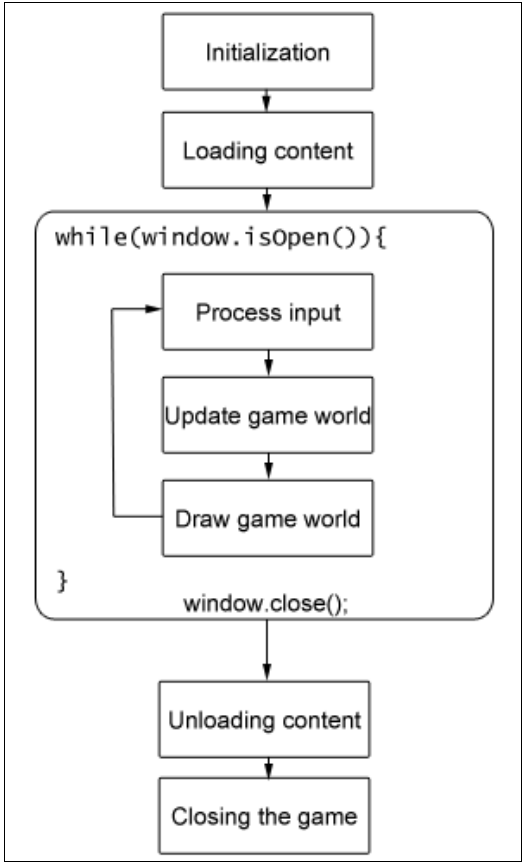
\includegraphics[scale=0.3]{graphics/sfml_basic}
    \caption{Basic structure of code in SFML}
    \label{fig:sfml_structure}
\end{figure}

\textbf{Basic SFML Drawing} 

\begin{minted}[bgcolor=lightgray]{cpp}
sf::RectangleShape rectangle(sf::Vector2f(128.0f,128.0f));
rectangle.setFillColor(sf::Color::Red);
rectangle.setPosition(320,240);
\end{minted}
sf::RectangleShape is a derived class of sf::Shape that inherits from
sf::Drawable, which is an abstract base class that all entities must inherit from
and implement its virtual methods in order to be able to be drawn on screen. It also
inherits from sf::Transformable, which provides all the necessary functionality in
order to move, scale, and rotate an entity. This relationship allows our rectangle to be
transformed, as well as rendered to the screen. In its constructor
a new data type: sf::Vector2f is introduced. It's essentially just a struct of two floats, x and y,that represent a point in a two-dimensional universe, not to be confused with the
std::vector, which is a data container.

The rectangle constructor takes a single argument of sf::Vector2f which represents
the size of the rectangle in pixels and is optional. On the second line,  the fill
color of the rectangle by providing one of SFML's predefined . Lastly,
the position of our shape by calling the setPosition method and passing its
position in pixels alongside the x and y axis, which in this case is the centre of our
window. There is only one more thing missing until we can draw the rectangle:

\begin{minted}[bgcolor=lightgray]{cpp}
window.draw(rectangle); 
\end{minted}

\textbf{Drawing Image in SFML}

To draw images in SFML, One needs to be familar with two class sf::Texture and sf::Sprite. 
A texture is simply a graphical image that is located in computer's storage. Any image can be turned into texture by loading it. 
\begin{minted}[bgcolor=lightgray]{cpp}
sf::Texture texture; 
texture.loadFromFile("filename.png"); 
\end{minted}

Now, the image has been loaded. It is time to turn it into sprite. A sprite, much like the sf::Shape derivatives we have worked with so far, is a sf::Drawable object, which in this case represents a sf::Texture and also supports a list of transformations, both physical and graphical. Think of it as a simple rectangle with a texture applied to it.\cite{Barbier(2015)} \cite{Pupius(2015)}

Since the image has already been loaded as a texture. Its very easy to create sprite:
\begin{minted}[bgcolor=lightgray]{cpp}
sf::Sprite sprite(texture); 
window.draw(sprite); 
\end{minted}


\section{Box2D}
\subsection{Introduction}
Box2D is one of the most popular 2D physics engines. It is light, robust, efficient and highly portable. It has been used by several applications in several platforms.

A physics engine simulates the physics of objects to give them believable real-life movement. Although it can be used for other applications, it is primarily used as a library for games, and games make up the majority of softwares using Box2D. The engine is written and maintained by Erin Catto and is easily accessible at: \url{https://github.com/erincatto/box2d} and one can visit \url{https://box2d.org/documentation} for documentation of different features of the engine.

\subsection{Core Concepts of Box2D}
\begin{enumerate}
  \item \textbf{World:} World manages the physics simulation. It knows everything about the overall coordinate space and also stores lists of every element in the world.
  
  \item \textbf{Body:} Body serves as the primary element in the Box2D world. It has a location and also has a velocity.
  
  \item \textbf{Shape:} Shape keeps track of all the necessary collision geometry attached to a body.
  
  \item \textbf{Fixture:} Fixture attaches a shape to a body and sets properties such as density, friction, and restitution.
  
  \item \textbf{Joint:} Joint acts as a connection between two bodies (or between one body and the world itself).
\end{enumerate}


\subsection{Creating a world and bodies}
To create world, first  a gravitational force for the world is created.

\begin{minted}[bgcolor=lightgray]{cpp}
b2Vec2 gravity(0.0f, -10.0f);
\end{minted}

Now  a world is created:
\begin{minted}[bgcolor=lightgray]{cpp}
b2World world(gravity);
\end{minted}

Bodies are made by first setting up a definition, and then using this to create the body object itself.
\begin{minted}[bgcolor=lightgray]{cpp}
  b2BodyDef myBodyDef; 
  myBodyDef.type = b2_dynamicBody; //this will be a dynamic body
  myBodyDef.position.Set(0, 20); //set the starting position
  myBodyDef.angle = 0; //set the starting angle
\end{minted}

\newpage

Now, let us use this definition to create the body instance: 
\begin{minted}[bgcolor=lightgray]{cpp}
  b2Body* dynamicBody = world->CreateBody(&myBodyDef);
\end{minted}

Here, the world variable is a b2World object. The world object is like the boss of everything in Box2D, it handles the creation and deletion of physics objects. A body is basically invisible, so if a program like this is built and run, there is nothing to see yet.

To give a body its size, shape, and other tangible characteristics, we add fixtures to it. Also, the default behaviour is that adding fixtures will affect the mass of the body too. A body can have many fixtures attached to it, each fixture added will affect the total mass of the body. For now, let us add one simple fixture to this body, a square, and look a bit further at fixtures in the next topic. 
  \begin{minted}[bgcolor=lightgray]{cpp}
  b2PolygonShape boxShape;
  boxShape.SetAsBox(1,1);
  b2FixtureDef boxFixtureDef;
  boxFixtureDef.shape = &boxShape;
  boxFixtureDef.density = 1;
  dynamicBody->CreateFixture(&boxFixtureDef)
  \end{minted}
  
  The body definition must also specify the “type” of body we want to make. There are three possibilities:

\begin{itemize}
    \item \textbf{Dynamic:} This is what we will use most often—a “fully simulated” body. A dynamic body moves around the world, collides with other bodies,        and responds to the forces in its environment.

    \item \textbf{Static:} A static body is one that cannot move (as if it had an infinite mass). We’ll use static bodies for fixed platforms and boundaries.

    \item \textbf{Kinematic:} A kinematic body can be moved manually by setting its velocity directly. If you have a user-controlled object in your world, you can use a kinematic body. Note that kinematic bodies collide only with dynamic bodies and not with other static or kinematic ones.
\end{itemize}

\end{document}